% This is samplepaper.tex, a sample chapter demonstrating the
% LLNCS macro package for Springer Computer Science proceedings;
% Version 2.21 of 2022/01/12
%
\documentclass[runningheads]{llncs}
%
\usepackage[T1]{fontenc}
% T1 fonts will be used to generate the final print and online PDFs,
% so please use T1 fonts in your manuscript whenever possible.
% Other font encondings may result in incorrect characters.
%
\usepackage{graphicx}
% Used for displaying a sample figure. If possible, figure files should
% be included in EPS format.
%
% If you use the hyperref package, please uncomment the following two lines
% to display URLs in blue roman font according to Springer's eBook style:
%\usepackage{color}
%\renewcommand\UrlFont{\color{blue}\rmfamily}
%\urlstyle{rm}
%
\usepackage{comment}
%\usepackage[dvipdfmx]{color}
\usepackage[colorlinks=true, allcolors=blue]{hyperref}
\begin{comment}
    

\usepackage{amsmath}
%\usepackage{amsthm}
%\usepackage[dvipdfmx]{graphicx}
%\graphicspath{{./pictures/}}
\usepackage[dvipdfmx]{color}
\usepackage[colorlinks=true, allcolors=blue]{hyperref}
\usepackage{comment}
\usepackage{amssymb}
\usepackage{mathrsfs}
\usepackage{algorithmic}
\usepackage{algorithm}
\usepackage{ifthen}
\usepackage{enumitem}
\newboolean{Draft}
\newboolean{Draft2}
\setboolean{Draft}{false} %図を挿入するならtrue
\setboolean{Draft2}{false} %付録を挿入するならtrue
\end{comment}

\begin{comment}
\theoremstyle{plain}
%\newtheorem{theorem}{Theorem}
\newtheorem{theorem*}{Theorem}
%\newtheorem{proposition}{Proposition}
\newtheorem{subroutine}{Subroutine}
%\newtheorem{lemma}{Lemma}
\newtheorem{cor}{Corollary}
\theoremstyle{definition}
%\newtheorem{definition}{Definition}
\newtheorem{definition*}{Definition}
\end{comment}



\begin{document}
%
\title{Designing various algorithms based on DAG-pathwidth}
%
%\titlerunning{Abbreviated paper title}
% If the paper title is too long for the running head, you can set
% an abbreviated paper title here
%
\begin{comment}
\author{First Author\inst{1}\orcidID{0000-1111-2222-3333} \and
Second Author\inst{2,3}\orcidID{1111-2222-3333-4444} \and
Third Author\inst{3}\orcidID{2222--3333-4444-5555}}
%
\authorrunning{F. Author et al.}
% First names are abbreviated in the running head.
% If there are more than two authors, 'et al.' is used.
%
\institute{Princeton University, Princeton NJ 08544, USA \and
Springer Heidelberg, Tiergartenstr. 17, 69121 Heidelberg, Germany
\email{lncs@springer.com}\\
\url{http://www.springer.com/gp/computer-science/lncs} \and
ABC Institute, Rupert-Karls-University Heidelberg, Heidelberg, Germany\\
\email{\{abc,lncs\}@uni-heidelberg.de}}
\end{comment}

\author{Jun Kawahara\inst{1}\orcidID{0000-1111-2222-3333} \and
Shinya Izu\inst{1}\orcidID{1111-2222-3333-4444}}
%
\authorrunning{J. Kawahara et al.}
% First names are abbreviated in the running head.
% If there are more than two authors, 'et al.' is used.
%
\institute{Princeton University, Princeton NJ 08544, USA \and
Springer Heidelberg, Tiergartenstr. 17, 69121 Heidelberg, Germany
\email{lncs@springer.com}\\
\url{http://www.springer.com/gp/computer-science/lncs} \and
ABC Institute, Rupert-Karls-University Heidelberg, Heidelberg, Germany\\
\email{\{abc,lncs\}@uni-heidelberg.de}}

%
\maketitle              % typeset the header of the contribution
%
\begin{abstract}
%The abstract should briefly summarize the contents of the paper in 150--250 words.

DAG (directed acyclic graph)-pathwidth is a parameter that measures how closely a directed graph resembles a directed path. This parameter provides a non-trivial width even for DAG, which is difficult to parameterize with directed pathwidth. DAG-pathwidth is useful for designing parameterized algorithms to solve NP-hard problems even on DAGs.

In this paper, we first design parameterized algorithms with DAG-pathwidth for various NP-hard problems even on DAGs. Specifically, we design fixed-parameter tractable (FPT) algorithms for the Directed Dominating Set Problem and the Max Leaf Outbranching Problem. Given a DAG with $n$ vertices and a DAG-path-decomposition of width $w$, both problems can be solved exactly in $O(2^w w n)$ time. Similarly, we propose parameterized algorithms for the Directed Steiner Tree Problem and the $k$-Disjoint Path Problem. 

Next, we design a polynomial-time approximation algorithm for DAG-pathwidth that achieves an $O(\log^2 n)$ approximation ratio. We further improve this ratio to $O(\log^{3/2} n)$ by demonstrating the equivalence between constructing DAG-path-decomposition and solving one-shot Black Pebbling game. 

It is known that computing DAG-pathwidth is NP-hard, and, as far as we know, no algorithm has been known for finding small DAG-pathwidth. In this paper, we also design an algorithm that, given an integer $k$ and DAG $G$ with $l$ roots and at most $d$ outdegree, either computes a DAG-path-decomposition of $G$ with width at most $O(l d^k)$ or provides an evidence that the DAG-pathwidth of $G$ is greater than $k$.

%For the Directed Steiner Tree Problem, where the terminal set size is $k$, we propose an FPT algorithm that computes an exact solution in $O(2^w (k + w)n + n^2)$ time. For the $k$-Disjoint Path Problem, we develop a parameterized algorithm that computes an exact solution in $O((k+1)^w (w^2 + k)n + n^2)$ time.

%Finally, we define a new parameter DAG-treewidth as a generalization of DAG-pathwidth. DAG-treewith is a parameter that measures how similar is the structure of a directed graph to that of a directed tree. We show that constructing an optimal DAG-tree-decomposition that minimizes DAG-treewidth is NP-hard. After that, we design an FPT algorithm for the Directed Dominating Set Problem in $O(2^w w^2 n)$ time, with the DAG-treewidth $w$ as a parameter.

\keywords{Graph algorithm \and Computational complexity \and Directed acyclic
graph \and Pathwidth.}
\end{abstract}
%
%
%
\section{First Section}
\subsection{A Subsection Sample}
Please note that the first paragraph of a section or subsection is
not indented. The first paragraph that follows a table, figure,
equation etc. does not need an indent, either.

Subsequent paragraphs, however, are indented.

\subsubsection{Sample Heading (Third Level)} Only two levels of
headings should be numbered. Lower level headings remain unnumbered;
they are formatted as run-in headings.

\paragraph{Sample Heading (Fourth Level)}
The contribution should contain no more than four levels of
headings. Table~\ref{tab1} gives a summary of all heading levels.

\begin{table}
\caption{Table captions should be placed above the
tables.}\label{tab1}
\begin{tabular}{|l|l|l|}
\hline
Heading level &  Example & Font size and style\\
\hline
Title (centered) &  {\Large\bfseries Lecture Notes} & 14 point, bold\\
1st-level heading &  {\large\bfseries 1 Introduction} & 12 point, bold\\
2nd-level heading & {\bfseries 2.1 Printing Area} & 10 point, bold\\
3rd-level heading & {\bfseries Run-in Heading in Bold.} Text follows & 10 point, bold\\
4th-level heading & {\itshape Lowest Level Heading.} Text follows & 10 point, italic\\
\hline
\end{tabular}
\end{table}


\noindent Displayed equations are centered and set on a separate
line.
\begin{equation}
x + y = z
\end{equation}
Please try to avoid rasterized images for line-art diagrams and
schemas. Whenever possible, use vector graphics instead (see
Fig.~\ref{fig1}).

\begin{figure}
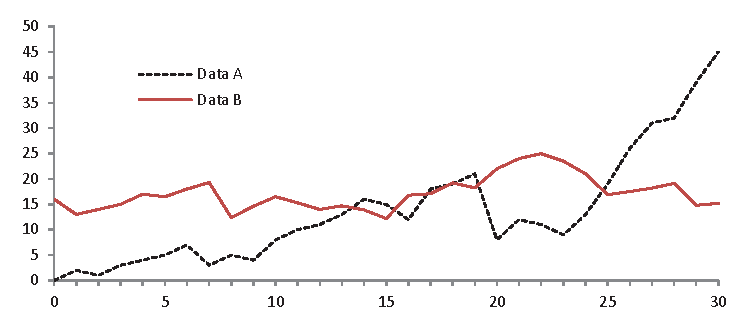
\includegraphics[width=\textwidth]{fig1.eps}
\caption{A figure caption is always placed below the illustration.
Please note that short captions are centered, while long ones are
justified by the macro package automatically.} \label{fig1}
\end{figure}

\begin{theorem}
This is a sample theorem. The run-in heading is set in bold, while
the following text appears in italics. Definitions, lemmas,
propositions, and corollaries are styled the same way.
\end{theorem}
%
% the environments 'definition', 'lemma', 'proposition', 'corollary',
% 'remark', and 'example' are defined in the LLNCS documentclass as well.
%
\begin{proof}
Proofs, examples, and remarks have the initial word in italics,
while the following text appears in normal font.
\end{proof}
For citations of references, we prefer the use of square brackets
and consecutive numbers. Citations using labels or the author/year
convention are also acceptable. The following bibliography provides
a sample reference list with entries for journal
articles~\cite{ref_article1}, an LNCS chapter~\cite{ref_lncs1}, a
book~\cite{ref_book1}, proceedings without editors~\cite{ref_proc1},
and a homepage~\cite{ref_url1}. Multiple citations are grouped
\cite{ref_article1,ref_lncs1,ref_book1},
\cite{ref_article1,ref_book1,ref_proc1,ref_url1}.

\begin{credits}
\subsubsection{\ackname} A bold run-in heading in small font size at the end of the paper is
used for general acknowledgments, for example: This study was funded
by X (grant number Y).

\subsubsection{\discintname}
It is now necessary to declare any competing interests or to specifically
state that the authors have no competing interests. Please place the
statement with a bold run-in heading in small font size beneath the
(optional) acknowledgments\footnote{If EquinOCS, our proceedings submission
system, is used, then the disclaimer can be provided directly in the system.},
for example: The authors have no competing interests to declare that are
relevant to the content of this article. Or: Author A has received research
grants from Company W. Author B has received a speaker honorarium from
Company X and owns stock in Company Y. Author C is a member of committee Z.
\end{credits}
%
% ---- Bibliography ----
%
% BibTeX users should specify bibliography style 'splncs04'.
% References will then be sorted and formatted in the correct style.
%
\nocite{*}
\bibliographystyle{splncs04}
\bibliography{mybibliography}
%

\begin{comment}
\begin{thebibliography}{8}
\bibitem{ref_article1}
Author, F.: Article title. Journal \textbf{2}(5), 99--110 (2016)

\bibitem{ref_lncs1}
Author, F., Author, S.: Title of a proceedings paper. In: Editor,
F., Editor, S. (eds.) CONFERENCE 2016, LNCS, vol. 9999, pp. 1--13.
Springer, Heidelberg (2016). \doi{10.10007/1234567890}

\bibitem{ref_book1}
Author, F., Author, S., Author, T.: Book title. 2nd edn. Publisher,
Location (1999)

\bibitem{ref_proc1}
Author, A.-B.: Contribution title. In: 9th International Proceedings
on Proceedings, pp. 1--2. Publisher, Location (2010)

\bibitem{ref_url1}
LNCS Homepage, \url{http://www.springer.com/lncs}, last accessed 2023/10/25
\end{thebibliography}
\end{comment}



\end{document}
